\documentclass[8pt]{beamer}
\usepackage[nobglogo]{beamerthemedmi-owled}
\usepackage[utf8x]{inputenc}
\usepackage{default}
\usepackage{url}
\usepackage{verbatim}
\usepackage{graphicx}
\usepackage{mathrsfs}
\usepackage{dl}
\usepackage{mls}
\usepackage[official]{eurosym}
\usepackage{fancyvrb}

%\usepackage{listings}


\mode<presentation>
{
  \usetheme{dmi-owled}
  %\usetheme{Warsaw}
  % or ...

  \setbeamercovered{transparent}
  % or whatever (possibly just delete it)
}

\title{Introduzione agli Open Data\\
Dati a 4 e 5 stelle\\
Interrogazioni e Vocabolari}

\author{Cristiano Longo\\ 
{\small{longo@dmi.unict.it}}}


\newcommand{\CNames}{N_C}
\newcommand{\PNames}{N_P}
\newcommand{\INames}{N_I}
\newcommand{\VNames}{V}

\newcommand{\Ont}{\mathcal{O}}
\newcommand{\Ontp}{\mathcal{O'}}
\newcommand{\literal}[2]{\mbox{``#1''\textasciicircum\textasciicircum\url{#2}}} % TODO
\newcommand{\literals}{\mathcal{L}}
\newcommand{\datatypes}{\mathcal{D}}
\newcommand{\stringLiteral}[1]{\mbox{``#1''}}

\date{Universit\`a di Catania}

\begin{document}
\maketitle
\setcounter{tocdepth}{1}

\section{Query}

\begin{frame}
\frametitle{Interrogazioni}

  Il metodo pi\`u immediato per ottenere informazioni da una ontologia \`e il 
  \emph{Conjunctive Query Answering}. Consideriamo ad esempio la seguente ontologia:

  \begin{tabular}{cc}
  \hline
  $\begin{array}{cl}
    \Ont  =  &  \{Female(Elise), Female(Alice), Male(Bob), \\
    &\phantom{\{}Male(Charlie), Male(Daniel), \\
    &\phantom{\{}Alice\,childOf\,Elise, Charlie\,childOf\,Elise, \\
    &\phantom{\{}Daniel\,childOf\,Alice, Daniel\,childOf\,Bob, \\
    &\phantom{\{}Francis\,childOf\,Charlie \}
  \end{array}$ & 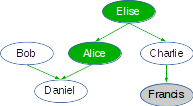
\includegraphics[width=120px]{family.png} \\
  \hline
  \end{tabular}

  Alcune interrogazioni che \`e possibile effettuare con il conjunctive query 
  answering sono:
  \begin{itemize}
    \item ``Trova tutti gli individui maschi.''
    \item ``Chi sono gli individui con almeno un figlio maschio?''
    \item ``Chi sono i figli di $Alice$?''
    \item ``Chi sono gli individui con almeno un figlio maschio ed una femmina?''
    \item ``Chi sono gli individui maschi con almeno un figlio maschio?''
  \end{itemize}
\end{frame}

\begin{frame}
  \frametitle{Query Congiuntive}
  Sia $\VNames = \{x, y, z, ... \}$ l'insieme infinito, numerabile 
  e disgiunto da $\CNames$, $\PNames$ e $\INames$ delle \emph{variabili}.
  Le \emph{formule atomiche} sono espressioni dei due seguenti tipi:
  \[
  C(x), \quad x\,P\,y
  \]
  con $x, y \in \INames \cup \VNames$, $C \in \CNames$ e $P \in \PNames$.
  \vspace{\baselineskip}

\uncover<2->{
  Una \emph{query congiuntiva} \`e una congiunzione finita di formule 
  atomiche $T_1 \wedge \ldots \wedge T_n$. Alcuni esempi ($x$ e $y$ variabili):
  \[
    Male(x); \quad y\,childOf\,x\,\wedge\,Male(y)  
  \]
}  
\end{frame}

\begin{frame}
  \frametitle{Query Congiuntive - Soluzione}
  
  Una soluzione per una query congiuntiva $Q=T_1 \wedge \ldots \wedge T_n$
  rispetto all'ontologia $\Ont$ \`e una sostituzione $\sigma$ che associa ad 
  ogni variabile in $Q$ un nome di individuo in $\Ont$ in maniera tale
  che le formule atomiche $\sigma T_1$, \ldots, $\sigma T_n$ compaiano
  tutte in $\Ont$.
  \vspace{\baselineskip}
  
\uncover<2->{  
  Consideriamo la query $Q$ e l'ontologia $\Ont$.
  \[
    Q=y\,childOf\,x\,\wedge\,Male(y)
  \]
  \begin{tabular}{lc}
    $\begin{array}{cl}
      \Ont  =  &  \{Female(Elise),  Female(Alice), Male(Bob), \\
      &\phantom{\{}Male(Charlie), Male(Daniel), \\
      &\phantom{\{}Alice\,childOf\,Elise, Charlie\,childOf\,Elise, \\
      &\phantom{\{}Daniel\,childOf\,Alice, Daniel\,childOf\,Bob, \\
      &\phantom{\{}Francis\,childOf\,Charlie \}\\
    \end{array}$ & 
    $\begin{array}{|c|c|}
      \hline
      x & y\\
      \hline
      Elise&Charlie\\
      Alice&Daniel\\
      Bob&Daniel\\
      \hline
    \end{array}$ \\
  \end{tabular}
}
\end{frame}

\begin{frame}
 \frametitle{Il protocollo SPARQL}
 Le basi di conoscenza presenti sul Web Semantico usualmente mettono 
 a disposizione uno \emph{SPARQL endpoint} che permette di interrogarle e,
 ove permesso, di modificarle.
 
 \begin{table}
 \begin{tabular}{|c|l|}
  \hline
  \bf{Knowledge Base} & \bf{Endpoint IRI} \\
  Europeana & \url{http://europeana.ontotext.com/sparql} \\
  CNR & \url{http://data.cnr.it/sparql/}\\
  Camera dei Deputati & \url{http://dati.camera.it/sparql}\\
  DBPedia & \url{http://dbpedia.org/sparql}\\
  \hline
 \end{tabular} 
 \caption{Alcuni endpoint sparql}
 \end{table}

\uncover<2->{
Il \emph{protocollo SPARQL} (vedi \url{http://www.w3.org/TR/sparql11-protocol/})
\`e basato sul protocollo HTTP le richieste SPARQL vengono inviate agli
endpoint come richieste GET o POST e l'endpoint risponde con un \emph{esito}.
\vspace{\baselineskip}
}

\uncover<3>{
Le richieste si suddividono in richieste di \emph{query} o \emph{update}.

In caso di richieste di tipo query effettuate con successo, la risposta alla
chiamata GET o POST conterr\`a anche tutte le \emph{soluzioni} dell'interrogazione
in uno dei formati XML, JSON o CSV (il formato di risposta va specificato 
nella richesta).
}
\end{frame}

\begin{frame}[fragile]
\frametitle{SPARQL Query Language}
Le richieste di tipo \emph{query} vanno specificate nel linguaggio
denominato \emph{SPARQL Query}.
%
La specifica di questo linguaggio \`e disponibile all'indirizzo
\begin{center}
 \url{http://www.w3.org/TR/sparql11-query/} .
\end{center}

Una \emph{query SPARQL} ha la seguente sintassi
\begin{Verbatim}[fontsize=\small]
BASE <iriBase>
PREFIX p1 : <iriP1>
...
PREFIX pn : <iriPn>

SELECT ?x1 ... ?xm WHERE { GraphPattern }
\end{Verbatim}
dove: 
\begin{itemize}
 \item la sezione $BASE\,<iriBase>$ \`e opzionale;
 \item $p1, \ldots, pn$ sono prefissi di namespace ($n\geq0$, se $n=0$ non \`e presente alcun prefisso);
 \item $<iriP1>, \ldots, <iriPn>$ sono IRI;
 \item $?x1, \ldots, ?xm$ sono \emph{variabili} ($m>0$);
 \item $GraphPattern$ \`e un \emph{graph pattern} di uno dei tipi che vedremo in seguito.
\end{itemize}
\end{frame}

\begin{frame}[fragile]
\frametitle{SPARQL Query Language - Triple Pattern}
Il tipo di graph pattern più basilare \`e quello dei \emph{triple pattern}.
Un triple pattern \`e una espressione di uno dei seguenti tipi:
\[
 s \, p \, o \,, \quad s \, \mathtt{a} \, o
\]
ove $s$ e $p$ possono essere IRI o variabili, \texttt{a} \`e una parola riservata, e $o$ pu\`o essere una
IRI, una variabile o un letterale.
\vspace{\baselineskip}

\uncover<2->{
  Le formule atomiche nelle query congiuntive possono essere facilmente tradotte in triple patterns:
  \begin{small}
  \[
    \begin{array}{lclr}
    C(?a) & \Longrightarrow & ?a\, \mathtt{a} \,C \quad | \quad ?a\, \mathtt{rdf:type}\, C \mbox{(le due formulazioni sono equivalenti)}\\    
    \\
    ?a\,P\,?b & \Longrightarrow & ?a\, P \,?b . 
    \end{array}
  \]
  \end{small}

  Si noti che la propriet\`a \texttt{rdf:type} viene utilizzata per esprimere l'appartenenza 
  nel linguaggio RDF.
\vspace{\baselineskip}
}

\uncover<3->{
  A differenza delle query congiuntive, in SPARQL le variabili possono comparire anche
  al posto del nome della classe o della propriet\`a. Ad esempio i seguenti due sono 
  triple pattern validi:
  
    \begin{small}
  \[
    \begin{array}{lr}
    ?C(a) & \mbox{``Trova tutte le classi cui appartiene }a\mbox{''}\\    
    \\
    ?a\,?p\,?b & \mbox{``Trova tutte le triple nell'ontologia''.}   
    \end{array}
  \]
  \end{small}
}
% Esempi di triple pattern sono
% 
% \begin{quote}
% ``Trova tutti gli individui maschi''
% \end{quote}
% \begin{Verbatim}[fontsize=\small]
% ?x rdf:type Male . 
% \end{Verbatim}
% 
% \begin{quote}
% ``Trova tutte le coppie [?x, ?y] in relazione \url{childOf}''
% \end{quote}
% \begin{Verbatim}[fontsize=\small]
% ?x childOf ?y . 
% \end{Verbatim}
\end{frame}

\begin{frame}[fragile]
\frametitle{SPARQL Query Language - Soluzioni}
Analogamente a quanto accade nell'ambito del conjunctive query answering,
le \emph{soluzioni} per un triple pattern $T$ rispetto a una ontologia $\Ont$ 
sono tutte le sostituzioni $\sigma$ che associano ad ogni variabile presente 
in $T$ una IRI o un letterale in modo tale che $\sigma T$ sia presente in $\Ont$.
\vspace{\baselineskip}

Il risultato di una query $Q$, avente come pattern un triple pattern $T$
e come variabili nella select $x_1, \ldots, x_n$,
rispetto all'ontologia $\Ont$ \`e l'insieme delle sostituzioni $\sigma$,
ristrette alle variabili $x_1, \ldots, x_n$, tali che
$\sigma T$ appartiene ad $\Ont$.
\end{frame}

\begin{frame}[fragile]
 \frametitle{SPARQL Query Language - Triple Pattern - Esempio}
 Consideriamo ad esempio la seguente ontologia (base prefix \url{http://ex.org/})
\begin{tabular}{cc}
$\begin{array}{cl}
  \Ont  =  &  \{Female(Elise), Female(Alice), Male(Bob), \\
  &\phantom{\{}Male(Charlie), Male(Daniel), \\
  &\phantom{\{}Alice\,childOf\,Elise, Charlie\,childOf\,Elise, \\
  &\phantom{\{}Daniel\,childOf\,Alice, Daniel\,childOf\,Bob, \\
  &\phantom{\{}Francis\,childOf\,Charlie \}
 \end{array}$ & 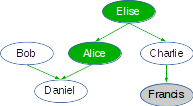
\includegraphics[width=120px]{family.png} \\
\end{tabular}

Consideriamo inoltre la query $Q$ definita come segue.

\begin{Verbatim}[fontsize=\small]
BASE <http://ex.org/>

SELECT ?x ?y WHERE { ?x childOf ?y . }
\end{Verbatim}

Le soluzioni di $Q$ rispetto a $\Ont$ sono
\begin{tabular}{|c|c|}
\hline 
?x & ?y \\
\hline
\url{<http://ex.org/Eliza>} & \url{<http://ex.org/Giorgia>} \\
\url{<http://ex.org/Eliza>} & \url{<http://ex.org/Francis>} \\
\hline 
\end{tabular}
\end{frame}

\begin{frame}[fragile]
 \frametitle{SPARQL Query Language - Basic Graph Pattern}
Un \emph{basic graph pattern} \`e un insieme di triple pattern, separati
dal carattere ``.''. Una sostituzione \`e una soluzione per un basic graph
pattern se e solo se \`e una soluzione per tutti i triple pattern
che compaiono in esso.
\vspace{\baselineskip}

Un esempio di query con il basic graph pattern \`e il seguente:
\begin{quote}
``Trova tutte le persone con almeno un figlo maschio''
\end{quote}
\begin{Verbatim}[fontsize=\small]
BASE <http://ex.org/>

SELECT ?x  WHERE { 
  ?y childOf ?x .
  ?y a Male
}
\end{Verbatim}
\vspace{\baselineskip}

\uncover<2->{
Da una query congiuntiva si pu\`o ottenere il basic graph pattern
corrispondente come segue:
\begin{itemize}
 \item applicare la trasformazione vista in precedenza ai triple pattern che lo costituiscono;
 \item sostituire i caratteri ``.'' con l'operatore logico di congiunzione $\wedge$.
\end{itemize}
Ad esempio
\[
 C(?x) \wedge ?x\,P\,b \quad \Longrightarrow \quad ?x\,\mathtt{a}\,C\,.\,?x\,P\,b\,.
\]
}
\end{frame}

\begin{frame}[fragile]
 \frametitle{SPARQL Query Language - Filtri sui letterali}
\`E possibile specificare dei filtri sui letterali che compaiono nei pattern.
Essi sono dei predicati, che dipendono dal tipo di dato dei letterali.\footnote{\url{http://www.w3.org/TR/sparql11-query/\#OperatorMapping}}
Permettono di selezionare tutte le soluzioni nelle quali ad una 
determinata variabile viene associato un letterale che soddisfa un predicato.
\vspace{\baselineskip}

La seguente query ad esempio permette di ottenere tutti
gli individui con un figlio il cui nome inizia con la lettera 'R'.
\begin{Verbatim}[fontsize=\small]
BASE <http://ex.org/>

SELECT ?x  WHERE { 
  ?y childOf ?x .
  ?y fullName ?name .
  FILTER regex(?name, "^R.*") .
}
\end{Verbatim}
\end{frame}

\begin{frame}[fragile]
 \frametitle{SPARQL Query Language - Optional Pattern Matching}

 Dati due graph pattern $P_1$ e $P_2$, il seguente \`e un \emph{optional graph pattern}:
\[
 P_1 \mathtt{OPTIONAL} P_2 .
\]

 Le sostituzioni che sono soluzioni per questo pattern sono quelle che
\begin{itemize}
 \item sono soluzioni per $P_1$ e $P_2$, oppure
 \item sono soluzioni per $P_1$
\end{itemize}
 
 sostitu
 
 
 SPC Data,\footnote{\url{http://spcdata.digitpa.gov.it/index.html}} tra le altre informazioni, contiene l'elenco di tutte le Pubbliche 
 Amministrazioni italiane. Le seguenti query permettono di ricavare la IRI 
 dell'individuo corrispondente al comune di Catania.\footnote{ NB:\url{fn:lower-case} \`e una funzione che converte un letterale
 in minuscolo.} 
 
\begin{Verbatim}[fontsize=\small]
SELECT ?x WHERE{
  ?x ?p "Comune di Catania"
} 

PREFIX fn: <http://www.w3.org/2005/xpath-functions#> 
SELECT ?x WHERE{
  ?x ?p ?l .
  FILTER (fn:contains(fn:lower-case(?l), "comune di catania"))
} 
\end{Verbatim}

La URL ottenuta come risultato \`e \emph{deferenceable}.
Visitandola col browser si ottiene una pagina web dove: vengono 
visualizzati tutti gli oggetti e i letterali con in quali
\`e in relazione, e le relative propriet\`a; tutte le classi cui appartiene, che sono
collegate all'individuo con la propriet\`a \texttt{rdf:type}.
\vspace{\baselineskip}

Da questo dataset \`e possibile ad esempio ottenere
tutti i comuni di una regione o l'elenco dei comuni e dei rispettivi
sindaci.
\end{frame}

\end{document}
